\section{真实链与理想链}

我们将粗粒化真实聚合物链转化为具有成键势和非成键势的“珠弹簧”链模型,聚合物骨架在介观尺度上的柔韧性应通过沿链相邻粒子间的成键势和非成键势的表达式表现出来。

在粗粒度链模型中,真实聚合物链的键合约束和相关的近邻势称为近程干扰,相对应的,远程干扰与聚合物段之间的相互作用有关,这些聚合物段沿着聚合物主干相隔很远,但在空间中距离很近。除此之外,远程干扰的一种典型表现就是所谓的“排斥体积效应”,即在空间中,一个盘绕的聚合物的任意两个片段不能占据相同的位置。

给出一个具体的粗粒链模型如下:

\begin{figure}[h]
\centering
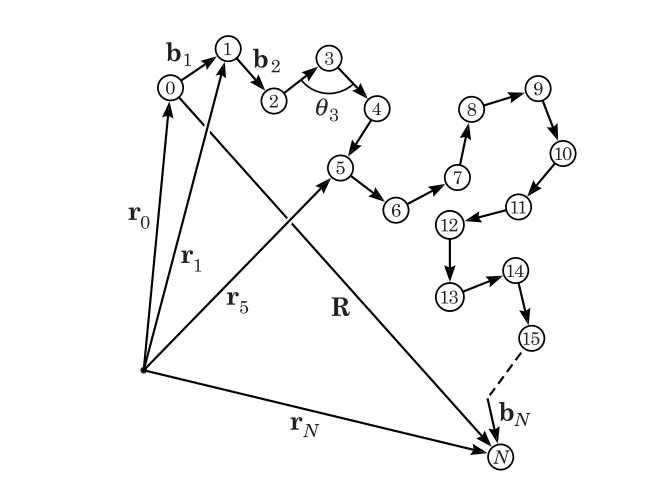
\includegraphics[scale=0.5
]{Contents/chapter2/figures/2-1.png}
\caption{粗粒链模型实例}
\end{figure}

此为由$N+1$个粒子与$N$个弹簧组成的粗粒链模型,粒子位置记为$\mathbf{r_0},……,\mathbf{r_N}$,键向量记为$\mathbf{b_1},……,\mathbf{b_N}$,链的端点间的向量记为$\mathbf{R}$。图中由2、3、4粒子的相互作用导致的$\theta_3$的角度限制就是一种近程干扰,而粒子6和12之间的穿透空间相互作用正说明了一种远程干扰。
从而,我们可以引出以下重要概念:
\begin{itemize}
	\item 真实链:考虑近程干扰和远程干扰的分子链。
	\item 理想链:仅考虑近程干扰而不考虑远程干扰的分子链。
\end{itemize}

有一个重要发现表示,不考虑近程干扰的特定形式,所有的理想链模型在足够大的长度范围内都具有普遍的缩放效应。为了更好的说明以上效应,考虑聚合物线圈的平均长度,$R=\sqrt{<\mathbf{R}\cdot \mathbf{R}>}$,其中$\mathbf{R}$为连接聚合物两端点的向量,符号$<……>$表示聚合物的全部构象态的平均值。从而,圈长$R$,即端点间向量的均方根,与聚合度N的关系如下
\begin{equation}
R \sim b N ^ { \nu } , \nu = 1 / 2 , \quad N \rightarrow \infty
\end{equation}
不考虑聚合物的化学细节和建模中使用的粗粒化水平,以上渐近比例关系中比例系数$\nu = 1/2$是通用的。非常值得注意的是,无论聚合物是聚苯乙烯还是聚乙烯,将聚合物链的分子量曾为四倍,聚合物线圈的平均尺寸就会增加一倍。相比之下,$(1)$式中作为前因子出现的长度尺度$b$(通常约为1nm)对聚合物的化学结构和粗粒化程度均敏感,但对总分子量不敏感。这个渐近极限的方法不是普遍的,它取决于近程干扰的范围。

从而我们考虑一个自然的问题,在什么条件下真实聚合物链满足$(1)$式中理想的链缩放定律?由于所有只有近程干扰的聚合物都表现出渐近理想的链缩放,这个问题可以转换为,在什么条件下真实链可以忽略远程干扰?令人好奇的是,线性均聚物在良好溶剂中无限稀释时的最简单情况并不遵循理想的链比例关系。

原则上,远程干扰永远不会完全消失。然而,通常会遇到两种情况,在这种情况下,远程干扰基本上可以忽略不计:
\begin{itemize}
	\item theta温度下高分子量均聚物的稀溶液。
	($\theta$态指溶液中高分子的链收缩和扩张力达到平衡,或溶剂与链段和链段与链段相互作用达到平衡,从而表观上呈现理想溶液的状态)
	\item 嵌在化学上相同的均聚物熔体中的均聚物链。
\end{itemize}

在排除了在空间上封闭但距离较远的聚合物段之间的体积相互作用的系统中,沿着这条链生成一个新的缩放行为的“通用性类”——即自避免随机游走:
\begin{equation}
R \sim b _ { s } N ^ { \nu } , \nu = 0.588 \ldots , \quad N \rightarrow \infty
\end{equation}
同样的,指数$\nu$是通用的,只取决于空间的维数(三维空间中$ v = 0.588 \dots$,二维空间中$ v =3/4 $),长度尺度$b_s$依赖于聚合物和溶剂的化学细节,但与聚合物分子量无关。
随着聚合物溶剂质量的降低(通常通过降低温度),聚合物段间的相互吸引作用通过溶剂介质传递。在$\theta$温度下,这些吸引相互作用正好补偿了排斥体积斥力,恢复了$(1)$式中的理想的链比例关系。

同样的现象也发生在均聚合物熔体中:两个聚合物段沿着同一条链远离,但在空间中间隔较短(约0.5 nm),它们之间的互斥很强。然而,这种净斥力在渐近极限过程中被许多其他的链(约有$N^{1/2}$个)抵消(“屏蔽”),这些链突出到兴趣链的随机线圈中。聚合物在相同聚合物熔体中的理想状态有时被称为弗洛里定理。

在这两种特殊情况以外的物理情况下,远程干扰通常在真实聚合物链的统计力学中起着重要的作用,应该通过指定合适的段间电位,将其纳入原子模型和介观模型中。我们将在第4章中看到,在构建粗粒度聚合物模型时,分离造成近程和远程干扰的相互作用是很方便的。此外,这种分离将产生聚合物场理论,其中单链模型的统计力学起中心作用。

读者可能已经注意到,对于在$(1),(2)$式中作为前置因子出现的非普遍长度$b$和$b_s$的物理解释一直相当模糊。粗略地说,我们可以把b看作是链的局部刚度损失和聚合物链的柔韧性首次显现的长度尺度。它与聚合物的键合约束的联系将在下面的具体理想链模型的背景下进行探讨。
